\startchapter{Mixture of Molecules} \label{ch:5}
\section{Description}

In Chapter \ref{ch:4}, experiments indicate that for one type of molecule at interfaces, even combining all the three spectral information, the constructed LP model cannot return the target composition in most cases. The existing spectral information is not adequate to obtain the target composition of one type of molecule at interfaces. Multiple return compositions can build the spectra that are almost exactly the same as the target ones. These compositions are returned by the LP models that use different amounts of spectral information. 


Because of the numerical limitation, each Lp model returns an optimal composition solution. It seems that our LP models have hit their limitation for the case of one molecule. However, there is another factor that is valuable to explore: the coordination of different molecules at interfaces. For a mixture of different molecules at interface, we want to figure out whether our LP models can help to obtain the target composition. If the LP models success in obtaining the target composition, then the rate of accuracy is the key factor of the study as well. \\

\section{Experiments}
To achieve the study of the coordination distribution of various molecules at interfaces, further experiments are constructed. These experiments have the following common settings. \\

First, there are six different amino-acids in the mixture: methionine, leucine, isoleucine(ile), alanine, threonine and valine. For each amino acid, only $\theta$ difference is considered, the other two Euler angles are integrated. Each amino acid molecule has 9 candidates in the mixture, they have $\theta$ of the following values: $0^{\circ}$,  $10^{\circ}$, $20^{\circ}$, $30^{\circ}$, $40^{\circ}$, $50^{\circ}$, $60^{\circ}$, $70^{\circ}$ and $80^{\circ}$. Because when $\theta$ equals $90^{\circ}$, the SFG spectra is a straight line. The corresponding candidate is excluded from all the experiments. As a result, there are 54 candidates in the mixture. \\

Second, the target composition need to be generated. The operation includes two steps: randomly pick one candidate from each amino acid's 9 candidates, and randomly generate a percentage for the selected candidate. The target composition is made of six randomly selected candidates coming from six different amino acids. The rest $48$ candidates have $0$ percentage in the target composition. Namely, six selected candidate makes 100\% component of the mixture. \\

Third, the IR, Raman and SFG spectra need to be generated for all the $54$ candidates and the target. \\

Each experiment in the experiment set contains different spectral information as shown in Table \ref{tab:5.1}. In Experiment 1, candidates' IR $x$ and $z$ polarization spectra are obtained. The target's IR $x$ and $z$ polarization spectra are generated by the dot product of the target composition and all the candidates' spectral data. Then the corresponding LP model is conducted using Equation \ref{eq:3.4}. Therefore, we claim that the LP model in Experiment 1 only contains IR information.\\

\begin{table}
\begin{center}
{\def\arraystretch{1.5}
\begin{tabular}{| l | p{3in} | }
\hline
Experiment Index & Spectral Information \\
\hline
Experiment 1 & $x$ and $z$ polarized IR spectra\\
\hline
Experiment 2 & $xx$, $xy$, $xz$ and $zz$ polarized Raman spectra \\
\hline
Experiment 3 & $yyz$, $yzy$ and $zzz$ polarized SFG spectra \\
\hline
Experiment 4 & $x$ and $z$ polarized IR spectra \newline $xx$, $xy$, $xz$ and $zz$ polarized Raman spectra \\
\hline
Experiment 5 & $x$ and $z$ polarized IR spectra \newline $yyz$, $yzy$ and $zzz$ polarized SFG spectra \\
\hline
Experiment 6 & $xx$, $xy$, $xz$ and $zz$ polarized Raman spectra \newline $yyz$, $yzy$ and $zzz$ polarized SFG spectra \\
\hline
Experiment 7 & $x$ and $z$ polarized IR spectra \newline
 $xx$, $xy$, $xz$ and $zz$ polarized Raman spectra \newline 
 $yyz$, $yzy$ and $zzz$ polarized SFG spectra \\
\hline
\end{tabular} 
}
\end{center}
\caption{Detailed experiment set setting} 
\label{tab:5.1} 
\end{table}	

Similarly, Experiment 2 contains only Raman spectral information of the following four polarizations: $xx$, $xy$, $xz$ and $zz$. Experiment 3 contains only SFG spectral information of $yyz$, $yzy$ and $zzz$ three polarizations. \\

Starting from Experiment 4, spectral information of different spectroscopy techniques are combined. In Experiment 4, IR spectral information is combined with Raman. In Experiment 5, IR spectral information is combined with SFG. In Experiment 6, Raman and SFG spectral information are incorporated. At the end, in Experiment 7, all three spectral information are put together: IR, Raman and SFG. \\

Each LP model of the experiments is using the same formula as shown in Equation \ref{eq:3.4}. Because every experiment is built with different spectral information, each LP model is conducted with different spectral information. \\

Finally, this experiment set is run 100 times in order to see which experiment in Table \ref{tab:5.1} return the target composition with the highest accuracy. This accuracy is measured by the time of each experiment returns the target composition. The scoring mechanism to measure whether a return composition matches to the target one is described in the next section. \\

\section{Scoring methods}

At the first glance, the sum of residuals between the spectra composed by the return composition and the target one can be used to measure the accuracy of the return composition. However, in most experiments conducted earlier, the spectra generated by the return composition are almost identical to the ones created by the target one. Therefore, this sum of residuals is negligible. It is not appropriate to use it as a scoring criteria. \\

Another way to measure the accuracy of the return composition, is to compare it directly with the target one. Therefore, calculating the sum of the residuals between a target composition and a return one directly is a faster approach to evaluate the accuracy of each experiment. The shortage of this approach is that it cannot be used to measure in real experiments where the target composition is unknown. However, in the current experiments, this approach can be a way to evaluate the return composition for all the mock experiments where the target compositions are known in advance. \\

The return composition of each experiment in the experiment set is obtained for each run. Each return composition is compared with the target one to calculate the sum of the residuals. If the sum is smaller than a certain threshold, which is $10^{-7}$. Then the return composition is considered to be the same as the target one. \\

\begin{figure}[!ht]
\centering
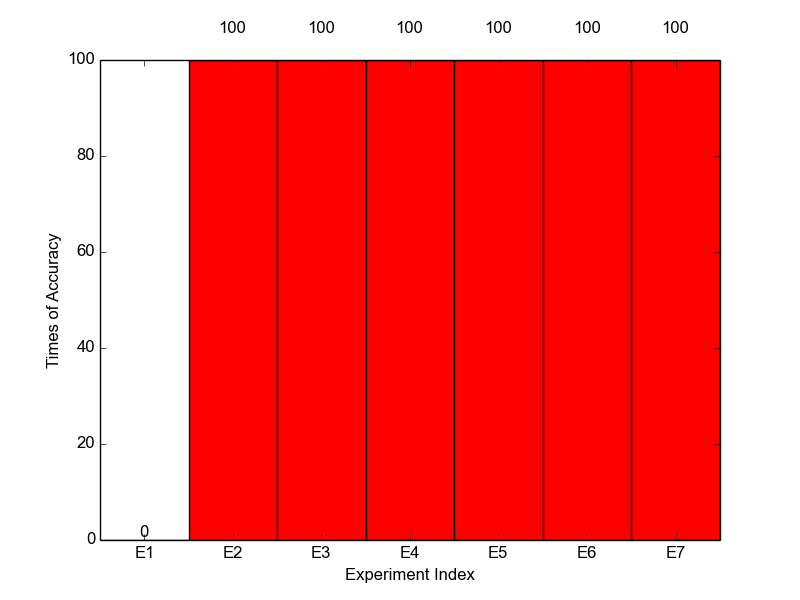
\includegraphics[scale=0.7]{Figures/accuracy_pecent_result8_mixture.png}
\caption{Accuracy analysis for experiments considering a mixture of amino acids with candidates from $0^{\circ}$ to $80^{\circ}$ on $\theta$ for each amino acid}  \label{fig:5.1}
\end{figure}

The experiment set is ran for 100 times, the result is shown in 
Figure \ref{fig:5.1}. In Experiment 2, the return composition of the LP model constructed by using Raman spectral information meets the target composition 100 times. This means that within this set of experiments, Raman is sufficient to obtain the correct composition of the target spectra. Moreover, the accuracy is 100\%. \\

Experiment 3 is the LP model constructed by using SFG spectral information. Its accuracy is 100\% as well. This indicates that SFG spectral information is as abundant as Raman for this set of experiments. \\

Experiment 4 to 7, each experiment contains either spectral information of Raman, or SFG, or both. Therefore, the corresponding LP model can help to get the target composition with the same accuracy as Experiment 2 and Experiment 3. \\

The only exception is Experiment 1. The accuracy is not as high as the other experiments. Its accuracy of the LP model that constructed using IR spectral information is $0$. The low performance can be caused by the insufficient spectral information of IR. \\

When this experiment set is re-run 100 times, only Experiment 1's returned composition is analyzed and focused. In each run, IR $x$ and $z$ polarized spectra are plotted both by the returned composition and the target one. The result is that these two polarizations' spectra conducted by the two different compositions are very close to each other in every run. For example, a random run is picked, then the two polarizations' spectra are plotted in Figure \ref{fig:5.2}. The spectra plotted by the return composition are almost the same as the ones plotted by the target composition. The residual is very small for the data points where these two spectra are not overlapped. This indicates that the optimum composition returned by the LP model conducted with only IR spectral information has achieved its best in obtaining a composition that best fit the target spectra. 

(TODO: rewrite or remove this paragraph) Comparatively, SFG has three unique polarizations, and Raman has four unique polarizations. From each projection's spectrum, we evenly select 200 data points. This means that one more projection will bring in 200 more constraints or 400 more (when we take the absolute sign off) constraints to the LP model. This would make a huge difference in the LP model, in term of further refining the candidate selection in target composition. However, it is still too early for us to say that Raman has more coordination information because it has four unique polarizations. Because for Raman's any polarization, the spectrum of candidate with $\theta$ equals to one degree is identical to the one of candidate with this $\theta$ degree's complementary. For example, the Raman spectra for candidate with $\theta$ of $10^{\circ}$, is the same as candidate with $\theta$ of $170^{\circ}$. And for IR, it is the same case. Only SFG tells the differences between these two degrees, as the spectra for candidate with $\theta$ of one degree is symmetric to its complementary along wavenumber as shown in Figure \ref{fig:5.8}. \\

\begin{figure}[!ht] 
\centering
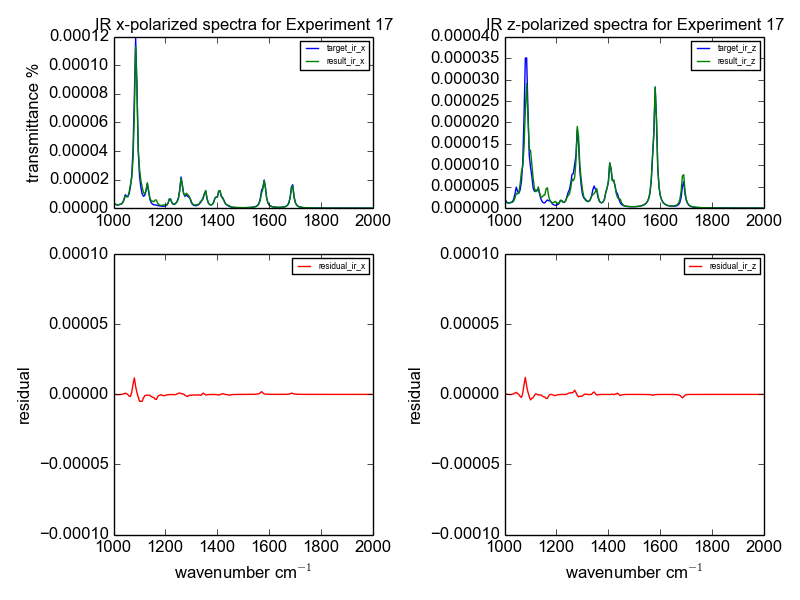
\includegraphics[scale=0.7]{Figures/chapter5_result_target_residual_plotting__ir_result8_run1.png}
\caption{IR Spectra Plotted by Result Composition and Target Composition.} \label{fig:5.2}
\end{figure}

To further study the capacity of the LP models built for the mixture of molecules,the candidate pool is expanded from $0^{\circ}$ to $180^{\circ}$ in terms of the $\theta$ value. Therefore, each amino acid has $18$ candidates. In total, there are $108$ candidates in the mixture. The same set of experiments in Table \ref{tab:5.1} is used. The only difference is randomly select one candidate from $18$ candidates, instead of $9$. All $108$ candidates' IR, Raman and SFG spectra need to be generated. Figure \ref{fig:5.3} illustrates the results obtained in $100$ runs. The accuracy in Experiment 1 is still low. This is not surprising as the complexity of the candidates has increased. Moreover, IR spectra for candidate with $\theta$ of one degree is identical to the one with $\theta$ of this degree's complementary, as shown in Figure \ref{fig:5.7}. This also increases the difficulty for the LP model constructed by using IR spectral information to return the target composition. \\

\begin{figure}[!ht]
\centering
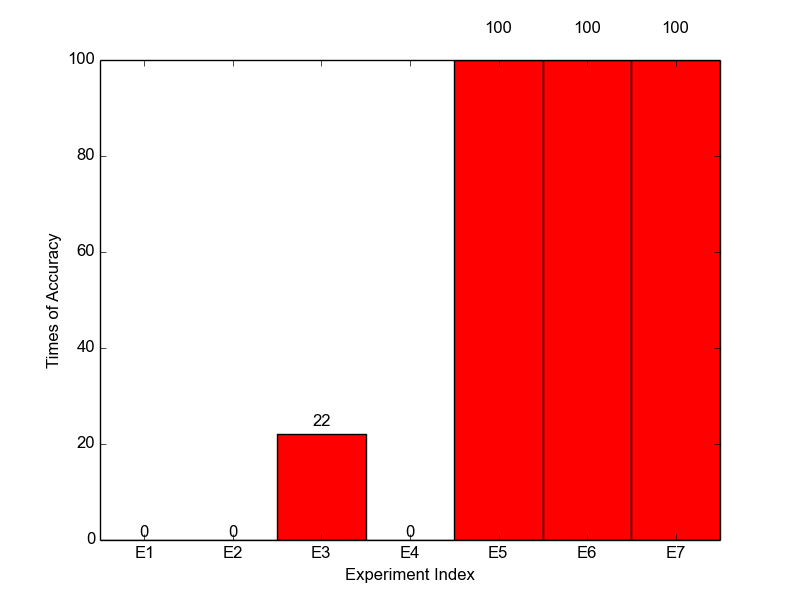
\includegraphics[scale=0.7]{Figures/accuracy_pecent_result10_mixture.png}
\caption{Accuracy analysis for experiments considering a mixture of amino acids with candidates from $0^{\circ}$ to $180^{\circ}$ on $\theta$ for each amino acid} \label{fig:5.3}
\end{figure}

However, it should be noticed that the accuracy for Experiment 2 has dramatically dropped. This is because the Raman spectra for one candidate with a $\theta$ is identical to the one of this $\theta$ value's complementary as displayed in Figure \ref{fig:5.8}. \\

In Figure \ref{fig:5.3}, the accuracy for Experiment 3 is no longer high neither. After increasing the number of amino acid candidates from $9$ to $18$, the complexity of the corresponding LP model has increased. From each projection, 200 data points are selected from the target and the candidates' spectra. Therefore, while the number of constraints is the same as before, the number of candidates are twice bigger than before. Although the added candidates' SFG spectra are symmetric along wavenumber which may greatly increase the uniqueness of the candidates as shown in Figure \ref{fig:5.9}. The spectral information is still insufficient to converge the composition to the target one. \\

The good result starts to emerge when using the combinations of IR and SFG or Raman and SFG. Figure \ref{fig:5.3} shows that Experiment 5, Experiment 6, Experiment 7 all have 100\% accuracies. This phenomenon can be explained as follow: SFG helps to distinguish a candidate from its complementary on $\theta$ value. The extra spectral information coming from IR or Raman helps to further refine the LP model, which can then converge the return composition to the target one. \\

Although the accuracy in Experiment 2 is low when each amino acid's candidates spread from $0^{\circ}$ to $180^{\circ}$ on $\theta$. There are still some noticable result in the return composition: for each amino acid, the percentage assigned is correct; however, the candidate presented may be the one with the correct degree, or the one with the correct degree's complementary. For example, a random run is selected. Figure \ref{fig:5.4} displays the target composition and Figure \ref{fig:5.5} displays the return composition of Experiment 2. Figure \ref{fig:5.6} is the return composition of Experiment 6. From the three figures, when extracting the non-zero values to generate a list, the three lists are the same. However, when overlapping Figure \ref{fig:5.4} with Figure  \ref{fig:5.5}, the position of each non-zero value is not identical. For example, value of $0.299586$ appears at $\theta$ of $150^{\circ}$ for Valine in Figure \ref{fig:5.4}. In Figure \ref{fig:5.5}, it appears at $\theta$ of $30^{\circ}$ for Valine. Same observation for values of $0.021196$, $0.00662804$, $0.000642609$, and $0.00789$ in Figure \ref{fig:5.4} and \ref{fig:5.5}. The LP model of Experiment 2 fails to tell which candidate is the exact one between the correct one and its complementary on $\theta$. This observation is a general case across all the experiment groups in the case of Experiment 2. From Experiment 6, as long as the spectra data from SFG is plugged into the LP model, the return composition is the same as the target one. \\

\begin{figure}[!ht] 
\centering
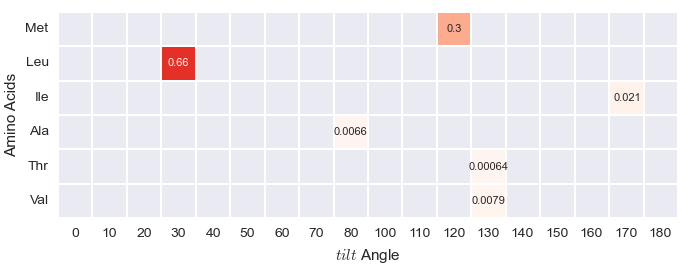
\includegraphics[scale=0.4]{Figures/mixture_target_composition_for_one_run_theta_0_180.png}
\caption{Target composition for one random run of six mixed amino acids with $\theta$ expanded from $0^{\circ}$ to $180^{\circ}$ on $\theta$} 
\label{fig:5.4}
\end{figure}

\begin{figure}[!ht] 
\centering
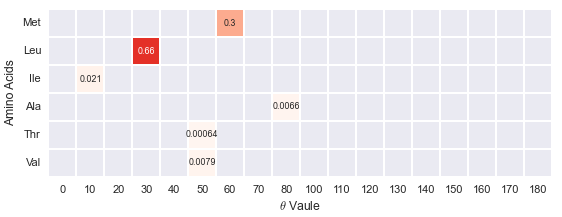
\includegraphics[scale=0.4]{Figures/mixture_return_composition_of_E1_for_one_run_theta_0_180.png}
\caption{return composition of experiment 2 for one random run of six mixed amino acids with $\theta$ expanded from $0^{\circ}$ to $180^{\circ}$ on $\theta$} 
\label{fig:5.5}
\end{figure}

\begin{figure}[!ht] 
\centering
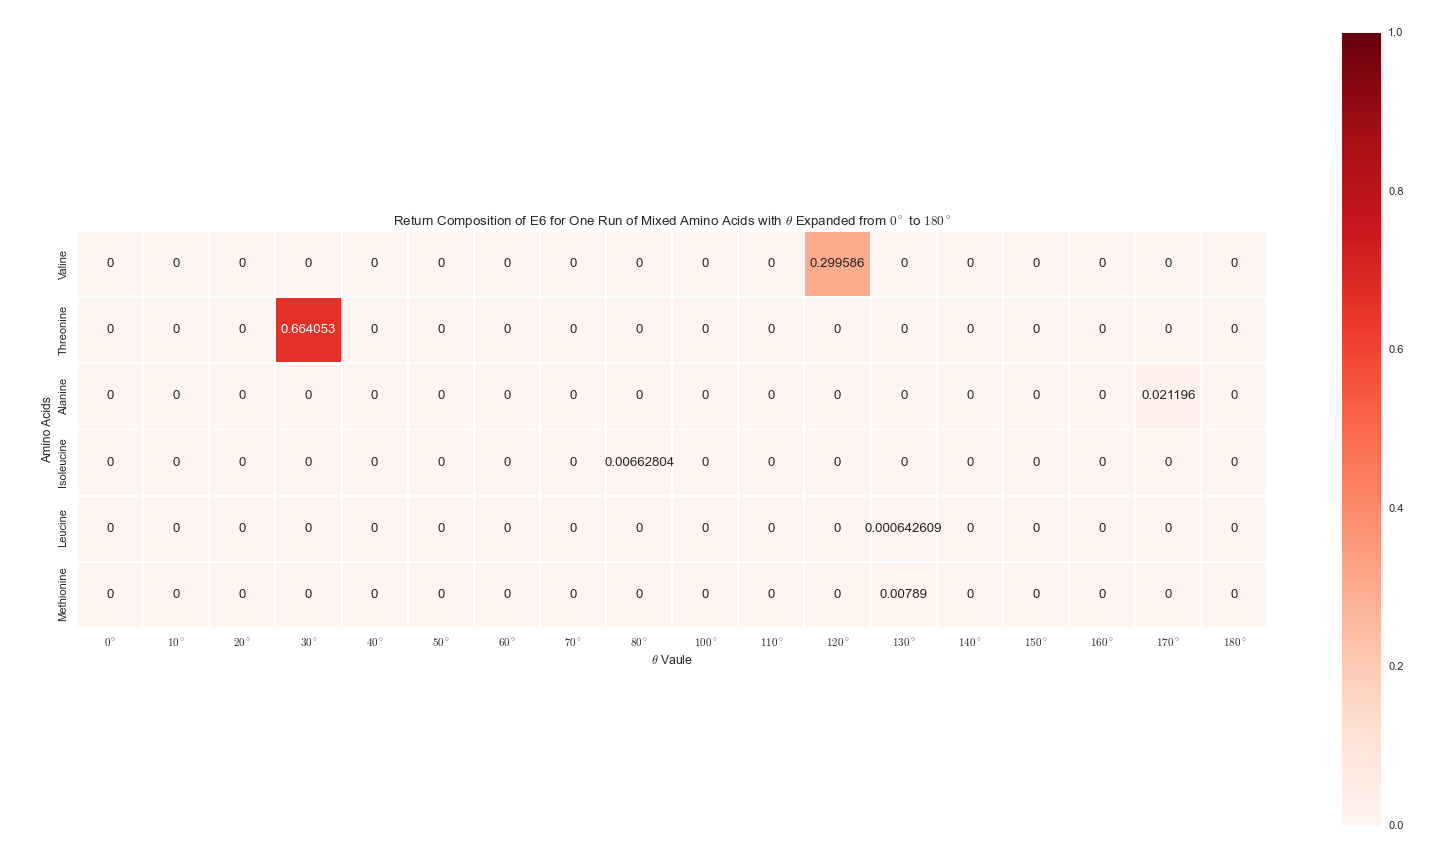
\includegraphics[scale=0.4]{Figures/mixture_return_composition_of_E6_for_one_run_theta_0_180.png}
\caption{return composition of experiment 6 for one random run of six mixed amino acids with $\theta$ expanded from $0^{\circ}$ to $180^{\circ}$ on $\theta$} 
\label{fig:5.6}
\end{figure}

From the above analysis, Experiment 2 appears the ability of limiting the number of candidates to $2$ for each amino acid. These two candidates are complementary on $\theta$ degree, with one of them to be the correct one for the target composition. The return composition of Experiment 4 is the same as the one of Experiment 2, which means combining IR spectra information with Raman is not sufficient for this experiments setting. Spectral information from SFG is needed in order to study the cases that having $\theta$ expanded from $0^{\circ}$ to $180^{\circ}$. \\


\begin{figure}[!ht] 
\centering
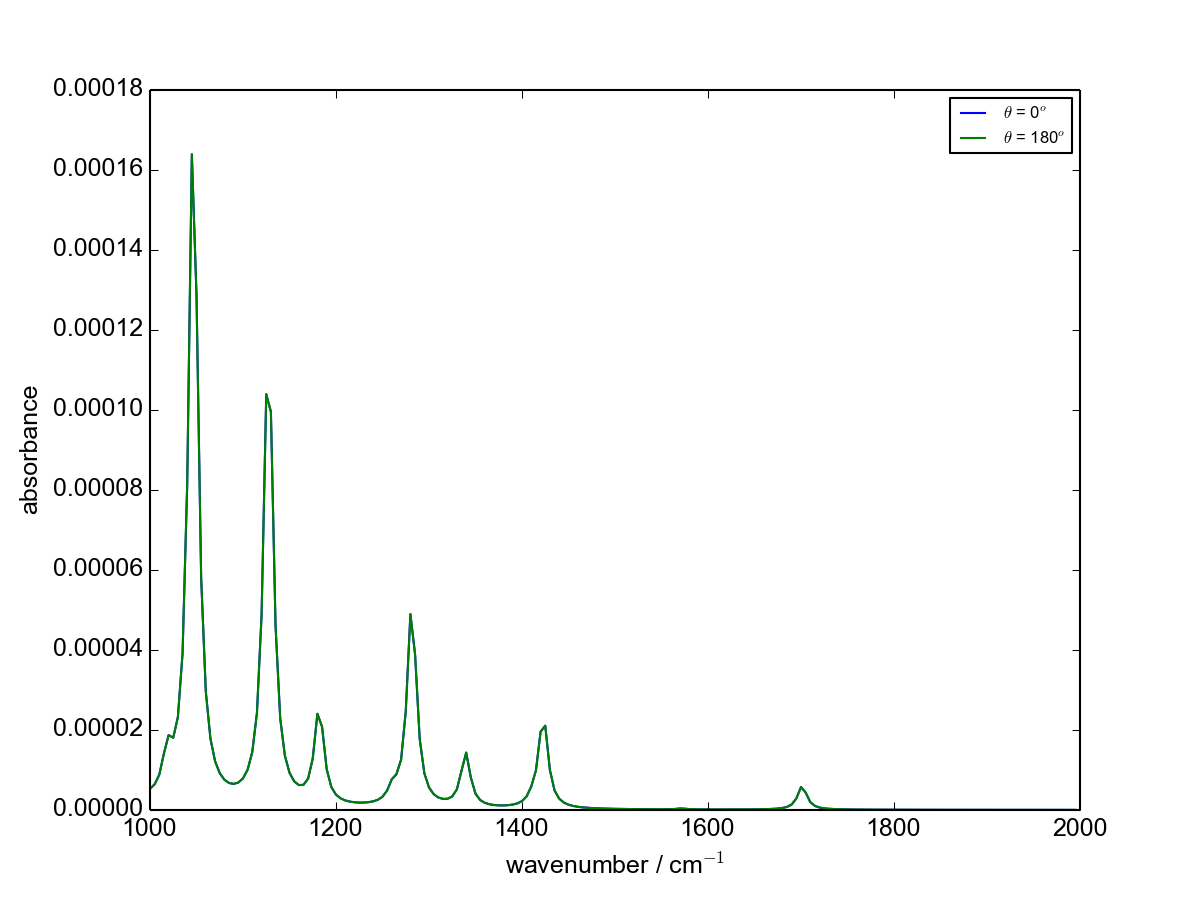
\includegraphics[scale=0.7]{Figures/Ala_candidates_plotting_ir_z_2.png}
\caption{IR $z$ projection spectrum for alanine candidate with $\theta$ of $0^{\circ}$ is identical to alanine candidate with $\theta$ of $180^{\circ}$} \label{fig:5.7}
\end{figure}

\begin{figure}[!ht] 
\centering
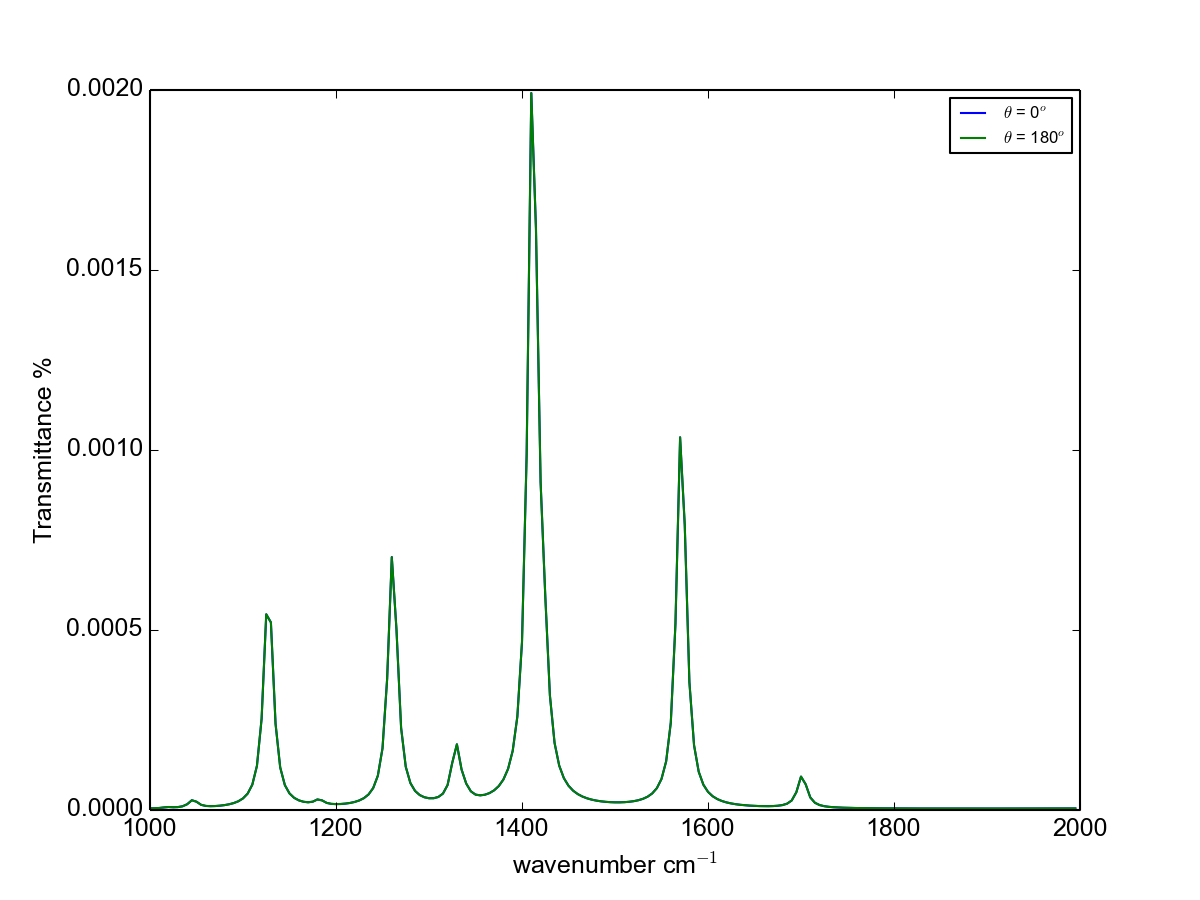
\includegraphics[scale=0.7]{Figures/Ala_candidates_plotting_raman_zz_2.png}
\caption{Raman $zz$ projection spectrum for alanine candidate with $\theta$ of $0^{\circ}$ is identical to alanine candidate with $\theta$ of $180^{\circ}$} \label{fig:5.8}
\end{figure}

\begin{figure}[!ht] 
\centering
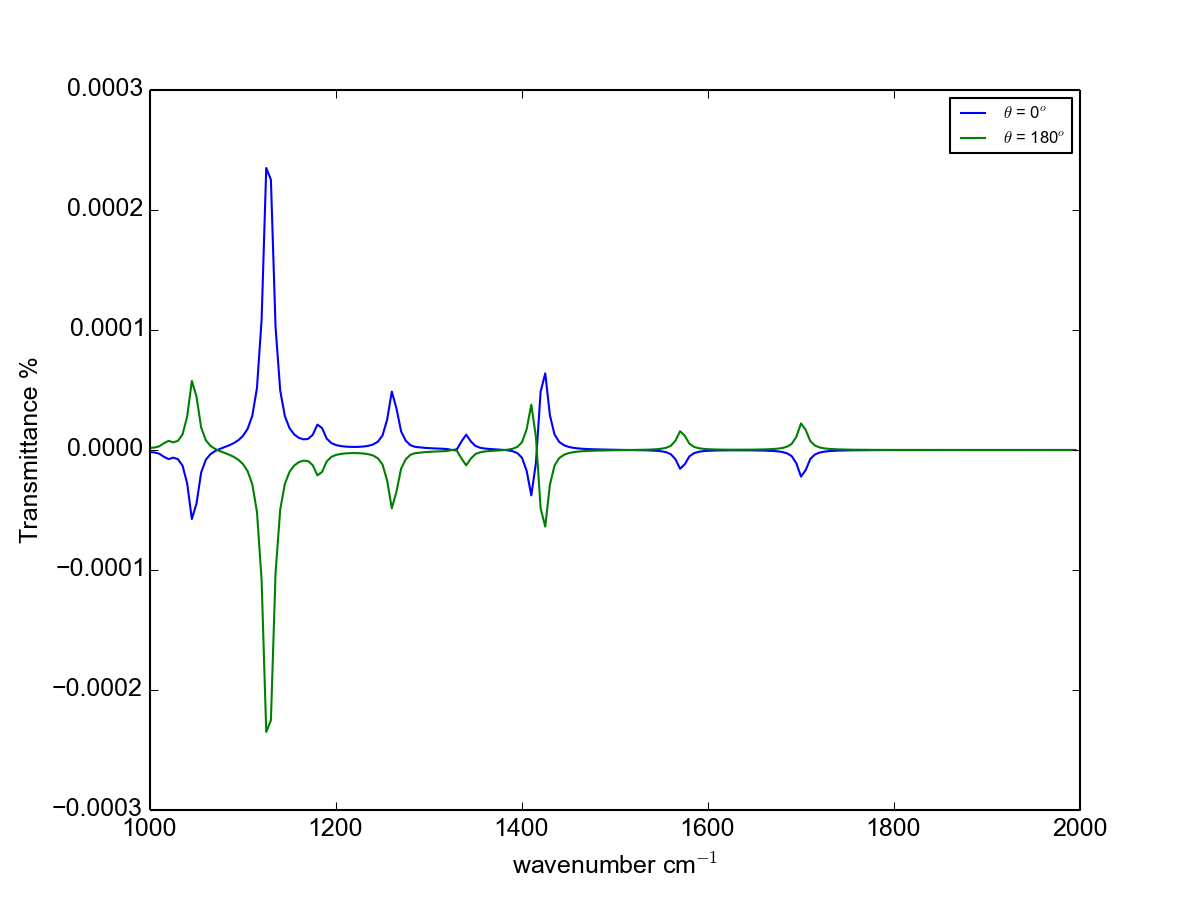
\includegraphics[scale=0.7]{Figures/Ala_candidates_plotting_sfg_zzz_2.png}
\caption{SFG $zzz$ projection spectrum for alanine candidate with $\theta$ of $0^{\circ}$ is not identical to alanine candidate with $\theta$ of $180^{\circ}$, but symmetric along wavelength} \label{fig:5.9}
\end{figure}
